\documentclass[conference]{IEEEtran}
\ifCLASSINFOpdf
  % \usepackage[pdftex]{graphicx}
  % declare the path(s) where your graphic files are
  % \graphicspath{{../pdf/}{../jpeg/}}
  % and their extensions so you won't have to specify these with
  % every instance of \includegraphics
  % \DeclareGraphicsExtensions{.pdf,.jpeg,.png}
\else
  % or other class option (dvipsone, dvipdf, if not using dvips). graphicx
  % will default to the driver specified in the system graphics.cfg if no
  % driver is specified.
  % \usepackage[dvips]{graphicx}
  % declare the path(s) where your graphic files are
  % \graphicspath{{../eps/}}
  % and their extensions so you won't have to specify these with
  % every instance of \includegraphics
  % \DeclareGraphicsExtensions{.eps}
\fi
\hyphenation{op-tical net-works semi-conduc-tor}

\usepackage{amsmath}
\usepackage{algorithm}  
\usepackage{algorithmic}
\usepackage{threeparttable}
\usepackage{graphicx}

\begin{document}

\title{A hybrid random-walk based web service recommendation enhanced by matrix factorization}

\author{
  \IEEEauthorblockN{Lin Jian}
  \IEEEauthorblockA{School of Physics and \\Electronic Information Engineering, \\WenZhou University\\
  Email: neolinjian@gmail.com}
  \and
  \IEEEauthorblockN{Homer Simpson}
  \IEEEauthorblockA{Twentieth Century Fox\\Springfield, USA\\
  Email: homer@thesimpsons.com}
}

\maketitle

\begin{abstract}
Recently, the QoS(Qaulity of Serivce) of Web Service that includes response-time, throughput and so on that needs more accuracy prediction. For many web service  callers, choosing the appropriate service in right time should be more significant events. So the web serivce recommendation is right to be the choice. The collaborative filtering is major approach to predict the QoS of more web service through the observed data. But the sparse density of data need new technology to enhance the accuracy of prediction. And the matrix factorization is aslo the common approach to solve the prediction. In this paper, we propose the new hybrid approach that combined the predictions with random-walk based and matrix factorization. Comprehensive experiments on the QoS data set of real-world web service, that our approach achieve the more accuracy predictions.
\end{abstract}

\begin{IEEEkeywords}
  random-work, web service recommendation, matrix factorization
\end{IEEEkeywords}

\IEEEpeerreviewmaketitle

%=========================================================================
\section{Introduction}
\par Overview the past few years, the collaborative filtering and matrix factorization have success in traditional fields of recommendation, such as Goods, Music, Moive and so on. The recommendation of web service was effected by the achievements. However, the scenario of web service is more complex that suffers from sparse data and incomplete related information. There are so many different web services distributing over heterogeneous network which contains several auto-systems. So the recommendation of web service should solve the problems that sparse QoS(Quality of Service) value collected from various with the intrusted infomation about location or network. In a word, more measures should be made to enhanced the limited information to achieve the more accuracy of web service recommendation. Only that, the system of web service can provide the more quality service.
\par Web Service QoS predicted information enhanced technology is developing fast. For example, time-aware recommendation that makes prediction by history call record, location-aware recommendation that make use of numbers of AS(auto system), IP or GPS(Global Position System). But the measures all achieve improvement in accuracy of prediction in small scale of the sparse data. Athough the information is critical to prediction, the experiments prove the factor that the more appropriate neighhorhood ranking can really boost the accuracy of prediction. So the paper that Random Walk Models can efficiently work in real-world datasets in the past year. With the transition probability matrix which based on the principle of markov random process, the undirected connected users can calculate the similarity in neighborhood selection.
\par In the field of web service recommendation, the random-walk model is efficient, but the accuracy of prediction needed more improvement. The matrix factorization had ever solved the sparse efficiently in similar scenario. Naturally, we will try combining the random-walk model with the matrix factorization to get the good performance. And the matrix factorization also is the best approach to reduction of dimensions, when we calculate the similarity between user and user, the time complexity will be smaller. With mroe high-efficiency model, the hybrid algorithm improve the accuracy of prediction in final.
\par  In summary, to solve the web service recommendation and to increase the accuracy of QoS prediction, in this paper, the contributions we made as following:
%=========================================================================
\begin{itemize}
\item We explore the extreme rate of data mining in known probability, and study the sparse density dataset and statistic phenomenon in real-world through calculation.
\item We propose the hybrid approach to combine the user-based collaborative filtering with matrix factorization.
\item We conduct the experiments on real-world datasets, and achieve the best accuracy of QoS prediction.
\end{itemize}

%=========================================================================
\par The rest of this paper is organized as follows. Section \ref{S-RW} summarizes the related work and our thought about sparse dataset. Section \ref{S-HRWMF} introduces our approach to combine the CF and MF algorithm. Section \ref{S-EE} reports the experiments and analyst the result of approaches. Section \ref{S-CN} concludes the paper and discusses the future work. 

%=========================================================================
\section{Related Work}\label{S-RW}
In this section, we will introduce the initiation of sparse density data, and explore the extreme rate of data mining in ideal environment that the sampling rate given in advance. Then the review of technology of recommendations will be displayed, includes collaborative filtering, matrix factorization, and random-walk model.

\subsection{Initition of the sparse density data}
\par In the real-world dataset environment, our recommendation system samples the whole dataset with $d \%$ density. Suppose that the matrix $Q$ have m users, n services, and the $Q\in \textbf{R}^{m\times n}$. $q_{ij}$ means the QoS of user i called service j. 
\par In our ideal sampling method that we suppose the system samples the data onto normal distribution. So the every user samples the QoS of service with number $n\times d  \% $. Athough the sampling method is ideal, the client user can implement the measure in the real environment. For example, with parameters $ m=300 , n=5000 , d\%=5\% $ , 300 users get $ 300 \times 5000 \times 5\% $ about $ 300 \times 250 $ QoS data from the dataset, and it can vividly reflected the sparse level from the fig1. And we can approximately calculate the expectation of number on the common invoked service number. Firstly, we suppose the $user_i$ samples the 250 service in whole, the $user_j (i \neq j)$ repeat the sampling process about 299 times. The model will subordinate to the binomial distribution of $X \sim b(299,0.05)$, and we can get the common invoke service number about $user_i$ by $E=np=14.95,D=np(1-p)=14.20$. So the real factor is the low sampling rate is hard to recover the data of whole, and the location-aware information is less affected the result of user-based collaborative filltering prediction.

\subsection{The extreme rate of data mining}
\par The extreme data mining rate maybe propose to solve our confusion that how the accuracy we can achieve by improve the recommended model. Maybe, we can use the statistic approaches to get the expectation about the extreme prediction. Finally, with the expectation we can improve our alogirthm to achieve more accuracy efficiently.
\par And the expectation of number about common invoked serivce is also the major latent factors in matrix factorization process. And Section \ref{S-EE} will displayed the relationship bewteen the best latent facters parameter and the matrix factorization accuracy. 

\subsection{User-based Collaborative Filtering}
The CF(Collaborative Filtering)-based algorithm have been widely used. The CF mines a user's common invoked services, which is identitied by response-time or throughput, by calculation of similarity (the Euclidean distance) between the $user_i$ and $user_j$.

\begin{equation}
dst(i,j)=\frac{1}{
  N_{ij}}\sqrt{\sum_{k \in S_{ij}}{(q_{ij}-q_{ij}})^{2}
} \label{eq1}
\end{equation}

where $S_{i,j}$ means the set includes the commonly invoked serivce by $user_{i}$ and $user_{j}$, and the $N_{ij}$ means the number of the common invoked service. By the Equcation (\ref{eq1}), we get the distance between two users, there is a defect that the two users have no common invoked serivce, the distance will be zero, we identity the smaller value  means the more similarity between two users, so the condition should be excluded in algorithm. 

\begin{equation}
sim(i,j)=\frac{1}{
  1+\frac{1}{N_{ij}}\sqrt{\sum_{k \in S_{ij}}{(q_{ij}-q_{ij}})^{2}}
}  \label{eq2}
\end{equation}
where the number 1 in the denominator is a way of Laplacian smooth to avoid the denominator being 0. It can conclude that the pair of users with the smaller distance is calcuated the value more near to number 1. In the reversed condition, the value will be number 0.

\par With the similarity calculated by front step. We can construct the similarity matrix $Sim \in \textbf{R}^{m\times m}$, the $s_{ij}$ means the similarity between $user_{i}$ and $user_{j}$. Then, we ranking the neighbors by cells of matrix, and choose the top K users to predict the QoS value with the Equcation (\ref{eq3}).

\begin{equation}
q^{'}_{ik}=\frac{
  \sum_{j \in TopK_{i}}{Sim_{ij} \times (Q_{jk}-\overline{Q_{j}})}
  }{
  \sum_{j \in TopK_{i}}{Sim_{ij}}
}+\overline{Q_{i}} 
\label{eq3}
\end{equation}
where $\overline{Q_{j}}$ means the average value of $user_{j}$, the Equcation (\ref{eq3}) also considers the different user has different baseline of QoS prediction. 

\subsection{Matrix Factorization}
The MF(Matrix Factorization) has also been chosen for its accuracy. By factorizing the matrix $Q \in \textbf{R}^{m \times n} $ into user and service latent matrix $U \in \textbf{R}^{m \times k}$, $S \in \textbf{R}^{n \times k}$. The decomposing process like  the Equcation (\ref{eq4})(\ref{eq5})(\ref{eq6}).

\begin{equation}
\begin{aligned}
\mathop{\arg\min}_{U,S} \sum_{i=1}^{m}{\sum_{j=1}^{n}{
(Q_{ij}-U_{i} \cdot S_{j}^{T}})^{2}
} \\
+ \lambda_{U} \cdot \sum_{i=1}^{m}\|U_{i}\|_{F}^{2}
+ \lambda_{S} \cdot \sum_{i=1}^{n}\|S_{i}\|_{F}^{2}
\label{eq4}
\end{aligned}
\end{equation}

\begin{equation}
{\frac{dloss}{dU_{i}}={\sum_{j=1}^{n}{
(Q_{ij}-U_{i} \cdot S_{j}^{T}}) \cdot S_{j}
} 
+ \lambda_{U} \cdot \|U_{i}\|
\label{eq5}
} 
\end{equation}

\begin{equation}
\frac{dloss}{dS_{j}}={\sum_{i=1}^{m}{
(Q_{ij}-U_{i} \cdot S_{j}^{T}}) \cdot U_{i}
}
+ \lambda_{S} \cdot \|S_{j}\|
\label{eq6}
\end{equation}

where the Equation (\ref{eq4}) is used to minimize the loss of equcation, and the $\| \cdot \|_{F}$ denotes the Frobenius norm to penalize the norms of U and S. The Equation (\ref{eq5}) (\ref{eq6}), we can use the gradient descent algorithm with several iterations, and find appropriate matrix U and S at last. Finally, the QoS value will be predicted by the inner product of $U_{i} \cdot S_{j}$. 
\par However, the matrix factorization is independent process, the latent matrix $U \in \textbf{R}^{m \times k}$ can be used as dimension reduction matrix of origin matrix $Q \in \textbf{R}^{m \times n}$, the dimension reduces from n to k. To some degree, the condition that user is with sparse records will be alleviated, and the the data in large scale will be dealt efficiently in short time.

\subsection{Random-Walk model}
\par The random-walk that based on PageRank alike measures (a Markov process) to get more appropriate neighbors ranking with the transition matrix.
\par In the last two Subsection, we get the matrix $Sim \in \textbf{R}^{m \times m}$, the $Sim_{ij}$ means the similarity between $user_{i}$ and $user_{j}$ by one step. As we all known, if $user_{i}$ and $user_{j}$ are undirected with one step,
the $user_{i}$ is similar to $user_{k}$ with similarity $Sim_{ik}$, and the $user_{j}$ is similar to $user_{k}$ with similarity $Sim_{jk}$, then we can achieve the similarity between  $user_{j}$ is similar to $user_{k}$ by two step. 
\par So we build the graph $G(V_{U},Sim)$ and use the Markov chain to model the state transition of random walk. Let $U_{0} \in V_{U}$ and the $Sim_{0,k}$ means the similarity between $user_{0}$ and the others. There are two choices for $user_{0}$:
\begin{itemize}
\item the $user_{0}$ with $\alpha$ probability by one step to link to itself.
\item the $user_{0}$ with $1- \alpha$ probability by one step to link to others.
\end{itemize}

The process goes by following equation.
\begin{equation}
P(X_{t}=j|X_{0}=i)=\left\{\begin{array}{ll}
\alpha ^{t} \cdot M^{t-1} \cdot Sim_{i}^{T}&i \neq j,\\
\alpha ^{t} \cdot M^{t-1} \cdot Sim_{i}^{T} + 1-\alpha &i = j.
\end{array}\right.
\end{equation}
The t steps random walking is 
\begin{equation}
P_{t}=(1-\alpha)P_{0}+ \alpha M^{T}P_{t-1} 
\label{eqrw}
\end{equation}
In summary, we have the transition matrix M. Along with the step t being infinite, the probability will converge to be stable, which is decided by the steday state distribution of the Markov chain. When the probability is stable, then the $P_{t}$ will equal to $P_{t-1}$, then the Equation \ref{eqrw} can be futher transformed into the following shape by linear algebra calculation.
\begin{equation}
P^{*}=(1-\alpha)(I-\alpha M^{T})^{-1}P_{0}
\label{eqrwfinal}
\end{equation} 
With the Equation \ref{eqrwfinal}, we can transform the matrix Sim more with more appropriate similarity value.

%=========================================================================
\section{Hybrid approach with RW and MF}\label{S-HRWMF}
\par The matrix Q will be decomposed into U and S which the latent dimension k at first. And the similarity matrix Sim will be calculated by $\frac{1}{k} \cdot U \cdot U^{T}$. Then the probabilistic matrix M will by calucate by following Equation:
\begin{equation}
M_{i,j}=\frac{Sim_{ij}}{\sum_{k \in Adj_{i}}{Sim_{ik}}}
\end{equation}
And the Equation (\ref{eqrwfinal}) will get the $P^{*}$ through the matrix M. 
\begin{equation}
\varphi_{i}=\frac{1}{N(j)} \cdot \sum_{j}{\frac{Sim_{ij}}{P^{*}_{ij}}} 
\end{equation}
The parameter $\varphi_{i}$ can easily calculated through Equation.
\begin{equation}
Sim_{ij}^{*}=\frac
{
\varphi_{i} \times P^{*}_{ij} + \varphi_{j} \times P^{*}_{ji}
}{2}
\end{equation}
With the new similarity matrix $Sim^{*}$ value, the top K nearest neighbors will be selected. 
\begin{equation}
\begin{aligned}
q_{ij}^{*}= \lambda \cdot (
\frac{
  \sum_{j \in TopK_{i}}{Sim_{ij} \times (Q_{jk}-\overline{Q_{j}})}
}{\sum_{j \in TopK_{i}}{Sim_{ij}}
}+\overline{Q_{i}}
) \\ + (1-\lambda) \cdot \sum_{k}U_{ik} \cdot S_{kj}
\label{final}
\end{aligned}
\end{equation}
The final QoS prediction will be calculated by Equation (\ref{final}). With the parameter $\lambda$, the predictions can adjust to different scenarios. The CF algorithm in sparse data will be more low than the real QoS value, and the MF algorithm will be more low high that the real QoS value with the regularizations. The overfitting or underfitting and changed by combine algorithm. The details of algorithm is in Algorithm \ref{alg_RWEMF}. And the code of algorithm could been found in WebSite \footnote{github.com/neoinmatrix/neosci/tree/master/rwemf}.
\begin{algorithm}  
\caption{the RWEMF}  
\label{alg_RWEMF}  
\begin{algorithmic}
\REQUIRE $Q$ , $\overline{U}$ ,$max\_iter$,$min\_thr$,$\lambda_{mf}$,$\lambda_{un}$,
\ENSURE $Q^{*}$
\STATE initialize $U_{i},S_{j}$ with random value
\STATE // decompose the matrix Q to U and S
\FOR {$t = 0$ to $max\_iter$}
    \STATE $U_{i} =U_{i}-(Q_{ij}-U_{i} \cdot S_{j}) -\lambda_{mf} U_{i}$
    \STATE $S_{i} =S_{j}-(Q_{ij}-U_{i} \cdot S_{j}) -\lambda_{mf} S_{i}$
    \STATE $loss=\sum{(Q_{ij}-U_{i} \cdot S_{j})}$
    \IF {$loss < min\_thr$} 
        \STATE break
    \ENDIF 
\ENDFOR
\STATE // calucate the similarity matrix 
\FOR {$i = 0$ to m}
    \FOR {$j = 0$ to m}
        \STATE $Sim_{ij}=\frac{1}{1+\frac{1}{N_{ij}}\sum{(U_{i}-U_{j})^2}}$
    \ENDFOR
\ENDFOR
\STATE // calucate the transtion matrix 
\FOR {$i = 0$ to m}
    \FOR {$j = 0$ to m}
        \STATE $M_{ij}=\frac{Sim_{ij}}{Sim_{i}}$
    \ENDFOR
\ENDFOR
\STATE // fix the similarity matrix with transtion matrix
\FOR {$i = 0$ to m}

    \FOR {$j = 0$ to m}
        \STATE $\varphi_{i}=\frac{1}{N(j)} \cdot \sum{\frac{Sim_{ij}}{P^{*}_{ij}}} $    
        \STATE $Sim_{ij}^{*}=\frac
{\varphi_{i} \times P^{*}_{ij} + \varphi_{j} \times P^{*}_{ji}
}{2}$
    \ENDFOR
\ENDFOR

\STATE // get the prediction by similarity matrix
\FOR {$i = 0$ to m}
    \FOR {$j = 0$ to m}
        \STATE $cf=\frac{
  \sum_{j \in TopK_{i}}{Sim_{ij} \times (Q_{jk}-\overline{Q_{j}})}
  }{
  \sum_{j \in TopK_{i}}{Sim_{ij}}
}+\overline{Q_{i}} $    
        \STATE $mf= U_{i} \cdot S_{j}$
        \STATE $Q_{ij}^{*}= \lambda_{un} \cdot cf + (1-\lambda_{un}) \cdot mf$
    \ENDFOR
\ENDFOR
\RETURN $Q^{*}$

\end{algorithmic}  
\end{algorithm}  
%=========================================================================
\section{Experiment and Evaluation}\label{S-EE}
\subsection{Dataset and Description}
The dataset is from WS-DREAM \footnote{github.com/wsdream/wsdream-dataset}. The whole dataset includes two attribute sub-datasets: response time(RT) and throughput(TP). The statistics of dataset are shown in Table \ref{tb1}. The dataset reflects the real-world condition that we have few clients to observe the QoS value and there are so many service on the Internet. 
% table=============================================
\begin{table}[H]
\begin{threeparttable}
\caption{Statistics of dataset}
\label{tb1}
\begin{tabular}{c||c|c|c|c|c|c} 
\hline 
QoS & numU & numS & min & max & mean & std \\ 
\hline 
RT(sec) & 339   & 5825  & 0.001 & 19.999 & 0.9086 & 1.9727 \\ 
\hline 
TP(kbps) & 339   & 5825  & 0.004 & 1000  & 47.5617 & 110.7971  \\ 
\hline 
\end{tabular} 
\end{threeparttable}
\end{table}

\par The information about the location of users and services can get in Table \ref{tb2}. The row of ``user\_as'' means there are 339 users in the dataset. And the 339 users are distributing in 136 areas. Every area has at least 1 user and no more than 31 users. And the average of users on one area about 2.4745 with 2.8338 standard deviation. Notice that the postfix ``\_as" and ``\_ct" means area is as(auto system) and ct(country) respectively. From the statistic information about data, the fact that users or services distribute in different area are extremely unbalanced. The location dataset provides inefficiency information, that is why the location information is hardly enhanced the accuracy of our experiments.

% table=============================================
\begin{table}[H]
\begin{threeparttable}
\caption{Statistics of userinfo and serviceinfo}
\label{tb2}
\begin{tabular}{c||c|c||c|c|c|c}
\hline 
infoattr & num & size & min & max & mean & std \\
\hline
user\_as & 339   & 136   & 1     & 31    & 2.4745 & 2.8338 \\
\hline
user\_ct & 339   & 30    & 1     & 161   & 10.9355 & 28.3673 \\
\hline
service\_as & 5825  & 992   & 1     & 1212  & 5.8661 & 40.6092 \\
\hline
service\_ct & 5825  & 73    & 1     & 2395  & 78.7162 & 285.9846 \\
\hline
\end{tabular} 
\end{threeparttable}
\end{table}

\subsection{Evaluation Metric and Parameter}
The MAE(Mean Absolute Error) and NMAE(Normalized Mean Absolute Error) may be the common measurable metrics. MAE is defined as 
\begin{equation}
MAE=\frac{1}{N}\sum_{i,j}{|q_{ij}-q^{\hat{}}_{ij}|}
\end{equation}
The NMAE is computed as the MAE normalized by the mean of all values, which is defined as 
\begin{equation}
NMAE=\frac{MAE}{\frac{1}{N}\sum_{i,j}{|q_{ij}}|}
\end{equation}
The MAE reflects the absolute error of the predictions. The NMAE reflects the relative error of the predictions. We can compare the ability of predictions from different dataset with NMAE relatively.

\subsection{Result Accuracy and Comparison}
\par There are several classical recommendation algorithms in the experiments as the comparisons. The result of response time and throughput
 are displayed in Table \ref{tb_rt} and Table \ref{tb_tp} respectively.
\par The comparisons including
\begin{itemize}
\item UPCC is the user-based collaborative filtering algorithm that calculate the similarity between users with Pearson correlation coefficient. In this case of small number of users, the algorithm is fast with short running time. 
\item IPCC is the user-based collaborative filtering algorithm that calculate the similarity between users with Pearson correlation coefficient. In this case of large number of services, the algorithm is slow with long running time. 
\item UIPCC is the hybrid method linearly combines the results of UPCC and IPCC, but the accuracy is more precise than that two. With the running time of total two algorithm, the algorithm is aslo slow.
\item PMF is the matrix factorization algorithm with the model of probability. In this case with sparse data, the process is fast to convergence stable state. So the maximum iteration and convergenced threshold are signifant to keep the running time within accepcteble range.
\item UL\_RWE is user-based random walk model enhanced by the matrix factorization. The dimension-reducted matrix U with k dimensions latent elements, the algorithm is more fast and achieve more accuracy.
\item RWEMF is our approach which are more efficient in the experiment. In the base of UL\_RWE, the approach successfully combined the matrix factorization prediction. The running time is close to matrix factorization to achieve more accuracy.
\end{itemize}

\begin{table}[H]
  \centering
  \caption{The MAE and NMAE of response time prediction}
  \label{tb_rt}
    \begin{tabular}{r||l|rrrr}
\hline
model & DS   & 5\%  & 10\% & 15\% & 20\% \\
\hline
UPCC & MAE  & 0.6159 & 0.5371 & 0.4966 & 0.4737 \\
         & NMAE & 0.6794 & 0.5917 & 0.5471 & 0.5219 \\
\hline
IPCC & MAE  & 0.6805 & 0.6572 & 0.5670 & 0.4955 \\
         & NMAE & 0.7507 & 0.7240 & 0.6246 & 0.5459 \\
\hline
UIPCC & MAE  & 0.6045 & 0.5336 & 0.4879 & 0.4601 \\
         & NMAE & 0.6668 & 0.5879 & 0.5374 & 0.5068 \\
\hline
PMF & MAE  & 0.5704 & 0.4894 & 0.4584 & 0.4390 \\
         & NMAE & 0.6292 & 0.5391 & 0.5050 & 0.4837 \\
\hline
UL-RWE & MAE  & 0.5255 & 0.4735 & 0.4462 & 0.4291 \\
         & NMAE & 0.5797 & 0.5216 & 0.4916 & 0.4727 \\
\hline
XEMF & MAE  & 0.5518 & 0.4891 & 0.4756 & 0.4877 \\
         & NMAE & 0.6087 & 0.5388 & 0.5239 & 0.5373 \\
\hline
RWEMF & MAE  & 0.5068 & 0.4560 & 0.4344 & 0.4251 \\
         & NMAE & 0.5591 & 0.5023 & 0.4786 & 0.4683 \\
\hline
    \end{tabular}
\end{table}


\begin{table}[H]
  \centering
  \caption{The MAE and NMAE of throughput prediction}
  \label{tb_tp}
    \begin{tabular}{r||l|rrrr}
\hline
model & DS & 5\% & 10\% & 15\% & 20\% \\
\hline
UPCC & MAE & 26.8039 & 22.2826 & 20.0274 & 18.689 \\
   & NMAE & 0.5643 & 0.4688 & 0.4212 & 0.3931 \\
\hline
IPCC & MAE & 29.5539 & 29.4531 & 30.1322 & 27.5450 \\
   & NMAE & 0.6222 & 0.6196 & 0.6338 & 0.5794 \\
\hline
UIPCC & MAE & 26.0401 & 21.9952 & 20.0911 & 18.6256 \\
   & NMAE & 0.5483 & 0.4627 & 0.4226 & 0.3918 \\
\hline
PMF & MAE & 22.5499 & 17.9761 & 16.5358 & 15.0594 \\
   & NMAE & 0.4748 & 0.3782 & 0.3478 & 0.3168 \\
\hline
UL-RWE & MAE & 19.4043 & 15.6509 & 14.3058 & 13.5797 \\
   & NMAE & 0.4085 & 0.3293 & 0.3009 & 0.2857 \\
\hline
XEMF & MAE & 21.0512 & 17.2567 & 15.9693 & 15.5798 \\
   & NMAE & 0.4432 & 0.3630 & 0.3359 & 0.3277 \\
\hline
RWEMF & MAE & 18.5121 & 15.1752 & 13.9855 & 13.3388 \\
   & NMAE & 0.3898 & 0.3193 & 0.2942 & 0.2806 \\
\hline
    \end{tabular}
\end{table}

\par Form the experimental results are shown in Table \ref{tb_rt} \ref{tb_tp}, we have some observations. 

\begin{itemize}
\item The matrix factorization algorithm(PMF) achieved more accuracy than the user-based or item-based without enhanced algorithm(UPCC,IPCC,UIPCC). 
\item The algorithm (HL-RWE) enhanced by random-walk model is achieve more accuracy than the similarity calculated based collaborative filtering algorithm(UPCC,IPCC,UIPCC). So the precision similarity calcualtion and the appropiate and ranking neignhbors seleceted are the efficient approaches to improve the accuracy.
\item The RWEMF algorithm is more efficient than other algorithms and achieves the best accuracy. The sparse density of 5\% is more appropiate for the algorithm to have accuracy that the dense density of 20\%.
\item In the different sub-dataset, the algorithms achieve different performance. The response-time dataset with value range (0.001-19.999) and standard deviation 1.9727 is with fluctuation about 9.86\%. The throughput dataset with value range (0.004-1000) and standard deviation 110.797 is with fluctuation about 11.08\%. The RWEMF achieves $\frac{0.6794-0.5591}{0.6794}=0.1771$ in rt dataset and $\frac{0.5643-0.3898}{0.5643}=0.3092$ in tp dataset. So the sparse density and the fluctuation in the dataset is the important elements to the RWEMF algorithm.
\end{itemize}

\subsection{Analysis and Deduction}
\par The signifcant parameters in RWEMF are top K, latent dimensions, the rate of mf union. 

\begin{figure}[H]  
\centering  
\includegraphics[width=0.45\paperwidth]{topk_rt.eps}  
\caption{the MAE of different topk of RWEMF on the response-time dataset }  
\label{fig_rt}  
\end{figure} 

\begin{figure}[H] 
\centering  
\includegraphics[width=0.45\paperwidth]{topk_tp.eps}  
\caption{the MAE of different topk of RWEMF on the throughput dataset }  
\label{fig_tp}  
\end{figure} 



\par From the Figure \ref{fig_rt} \ref{fig_tp}, the nearby neighbors selected obviously effects the mae accuracy. when topk=3, the RWEMF achieves the best accuracy in both response-time and throughput dataset. 

\par From the Figure \ref{fig_rumf_rt} \ref{fig_rumf_tp}, the rumf parameter is the rate united the mf. In the experiments, we choose the 5\% and 20\% density. And every rate of density has three lines including the rwe line ,mf line and rwemf line. It is clearly to know, the MAE of mf is largest in three, the MAE of rwe is smaller than mf's, with the 0.7 of rumf, the rwemf reaches the best accuracy of MAE. The phenomenon in the throughput dataset is similar. But the response-time dataset with small value is more sensitive to the rate, and it reaches the best accuracy in short range. 


\begin{figure}[H] 
\centering  
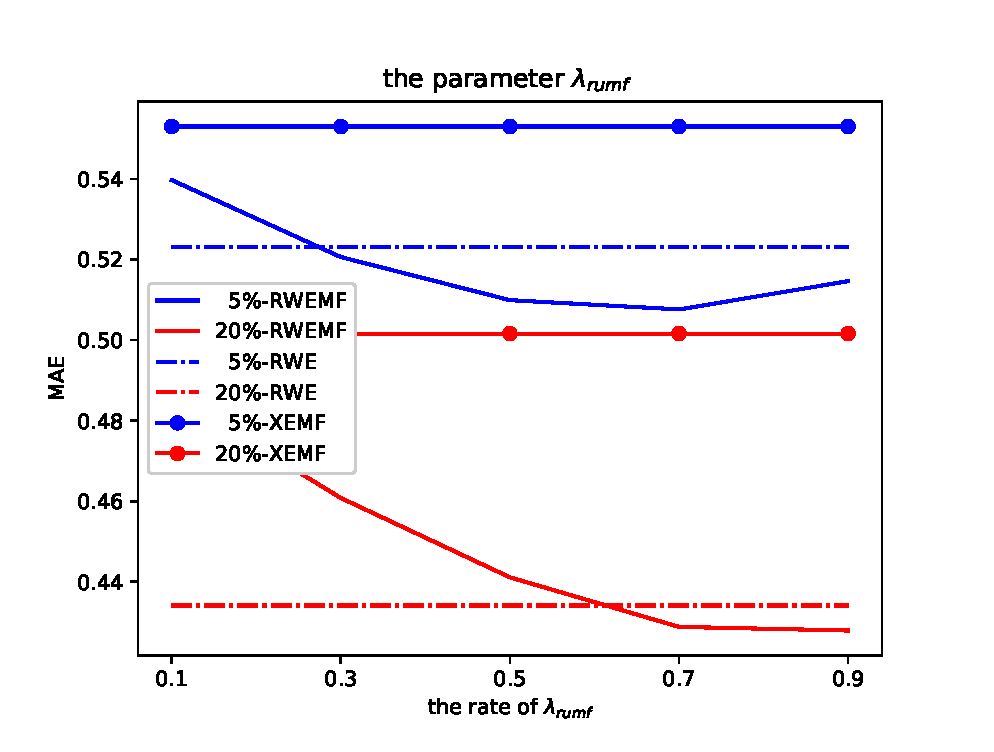
\includegraphics[width=0.45\paperwidth]{rumf_rt.eps}  
\caption{the MAE of different rate union mf on the response-time dataset }  
\label{fig_rumf_rt}  
\end{figure} 

\begin{figure}[H] 
\centering  
\includegraphics[width=0.45\paperwidth]{rumf_tp.eps}  
\caption{the MAE of different rate union mf  on the throughput dataset }  
\label{fig_rumf_tp}  
\end{figure} 

\par Every point in Figure \ref{fig_ae_rt} \ref{fig_ae_tp} means the prediction of RWEMF,RWE,MF three algorithm minus the real QoS value of dataset, and the points in view are sampling randomly that on behalf of the whole predicitons. It is easy to see the AE(Absolute Error) of RWEMF is locating in the middle between RWE's and MF's. Sometimes, the RWE can get the accuracy, but it also processes with the big variance. And the ME can not get the accuracy, but it aslo runs steadily with the small variance. And the predictions of algoithms are sensitive to value of dataset. The absolute error in throughput dataset fluctuated in large range compared to response-time dataset's.

\begin{figure}[H] 
\centering  
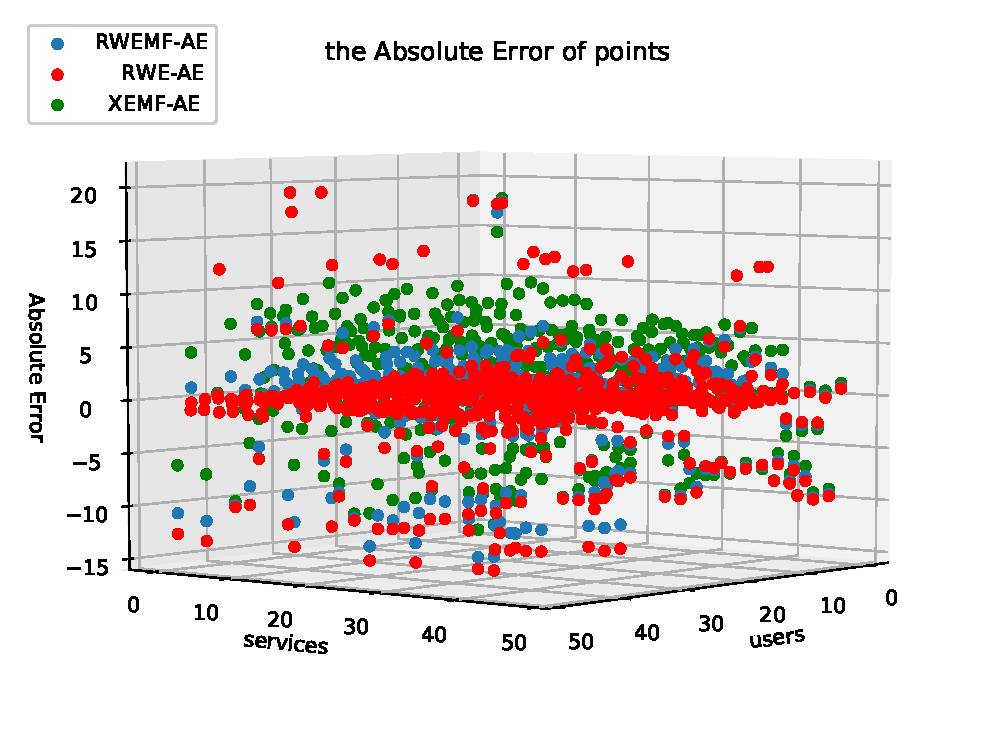
\includegraphics[width=0.45\paperwidth]{ae_rt.eps}  
\caption{the Absolute Error on the response-time dataset }  
\label{fig_ae_rt}  
\end{figure} 

\begin{figure}[H] 
\centering  
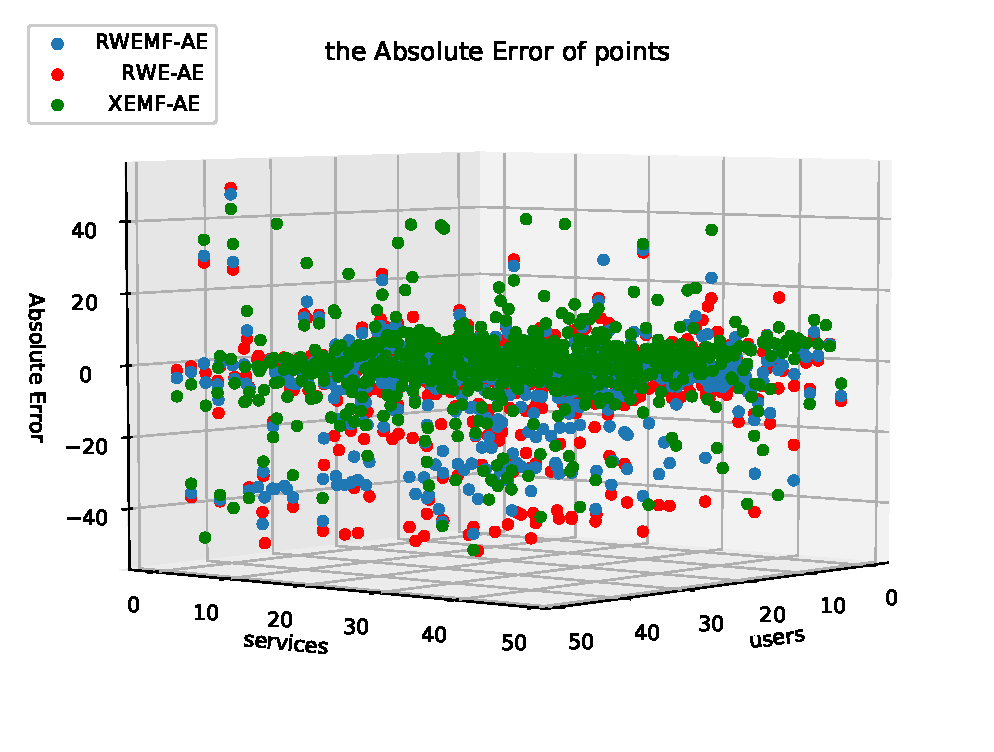
\includegraphics[width=0.45\paperwidth]{ae_tp.eps}  
\caption{the Absolute Error on the throughput dataset }  
\label{fig_ae_tp}  
\end{figure} 

%=========================================================================
\section{Conclusion}\label{S-CN}
\par We propose the RWEMF a hybrid approach to best accuracy in QoS real-world web service dataset. Firstly, We explore the sparse density dataset through statistic calculation. Clearly, the similar calculation and the nearby neighbors selection are significant. And the combination of random-walk user-based collaborative filtering and matrix factorization algorithm is described in the papers. The experiments of RWEMF prove our algorithm is most efficient and the best parameters chosen made RWEMF achieved the best accuracy in this QoS dataset.
\par In the future, with the best accuracy in this dataset, the RWEMF can be extended by more efficient model. The short running time and exquisite mind can help the algorithm using in real-world web service recommendation easily. The parameters for the hybrid model need more exploration and more study to keep the algorithm more efficient.Athough the adherent users's and service's infomation impove the accuracy finitely, there are more latent information value should be mined in the dataset. The MAE in 5\% on response-time dataset is 0.5068 now, athough the value is relative, sometime it could be metrics to measure the ability of algorithm in sparse dataset. Futhre, the MAE could be lower that 0.5000 by the new hybrid model.

%=========================================================================
\section*{Acknowledgment}
The authors would like to thank...
\cite{lo_extended_2012}
\cite{lee_algorithms_2000}
\cite{chen_web_2014}
\cite{liu_location-aware_2016}
\cite{yin_network_2017}
\cite{zhang_exploring_2011}
\cite{li_kuang_personalized_2012}.

\bibliographystyle{IEEEtran}
\bibliography{IEEEabrv,rwemfbib}

% \begin{thebibliography}{1}
% \input{rwemfbib.bib}
% % \bibitem{IEEEhowto:kopka}
% % H.~Kopka and P.~W. Daly, \emph{A Guide to \LaTeX}, 3rd~ed.\hskip 1em plus
% %   0.5em minus 0.4em\relax Harlow, England: Addison-Wesley, 1999.

% \end{thebibliography}

\end{document}

